\subsection{Kort}
\label{sub:kort}

\begin{figure}
  \centering
  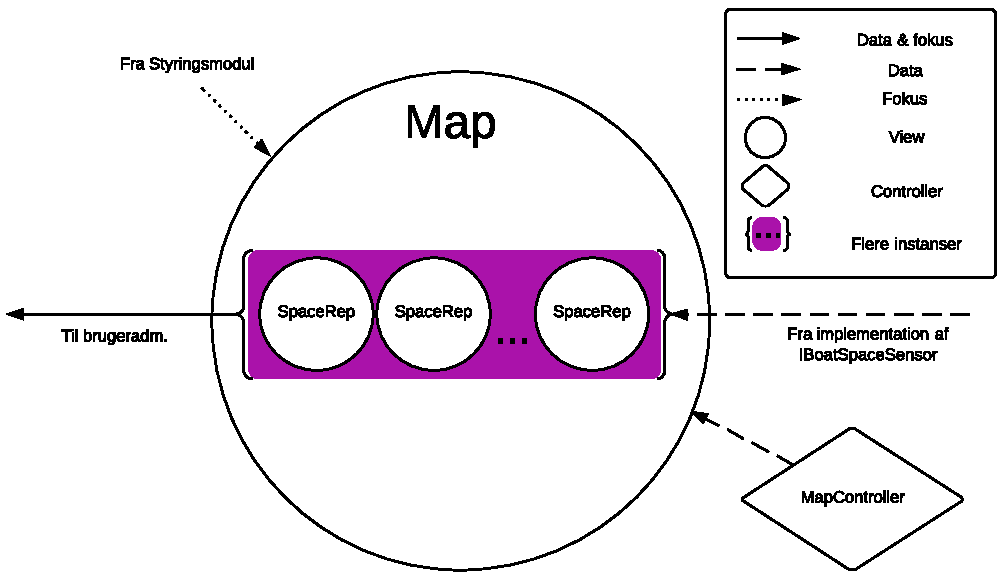
\includegraphics[width=\textwidth]{map-diagram.pdf}
  \caption{Oversigt over kort modulet.}
  \label{fig:map_diagram}
\end{figure}

Kortmodulet har til opgave at lave et kort, der giver et visuelt overblik over alle bådpladser der eksisterer på en havn.

\subsubsection{Funktionalitet}
\label{ssub:kort_funktionalitet}

Kortet præsenterer bådpladsers status i form af en beskrivende farve. Eksempelvis er en optaget bådplads status repræsenteret med farven rød, imens en fri bådplads status repræsenteres med farven grøn. Kortet skal modellere virkeligheden, således at virkelighedens informationer er reflekteret i kortet. Hvis et andet modul ændrer en bådplads status, skal dette modul skifte bådplads beskrivende farve til den tilsvarende.

\subsubsection{Implementation}
\label{ssub:kort_implementation}

Kortet kan tilgås fra styringsmodulet, som det fremstår på \cref{fig:map_diagram}. Det implementerede kort er opbygget af to grafiske lag. Et statisk baggrundslag, som viser havnens broer. Dertil et overliggende lag bestående af bådpladsrepræsentationer, \enquote{SpaceRep} i diagrammet, der er placeret på baggrundslaget, i forhold til deres beliggenhed. Det overliggende lag, \enquote{Map} i diagrammet, bliver oprettet af MapController, der også tildeler både til pladserne. En bådpladsrepræsentation er en reference til en bådplads i databasen. Når en sensor, der implementerer IBoatSpaceSensor, ændrer bådpladsens status i modellen, ændres repræsentation sig i takt, via modellen. Mere information omkring sensorer kan ses i \cref{sub:map_sensor_interface}

Når der klikkes på en bådplads på kortet, kan følgende scenarier ske, afhængigt af hvilken bruger der klikker.

\begin{tabu} to \textwidth {XX}
  \toprule
  \textbf{Tilstand} & \textbf{Reaktion} \\
   \midrule
   Brugeren ligger selv ved bådpladsen & Brugeren bliver videresendt til et modul der viser oplysninger om brugeren \\
   \midrule
  Der ligger en anden bruger på bådpladsen, og brugeren har de nødvendige adgangstilladelser & Brugeren videresendes, til et modul der viser oplysninger om brugeren \\
  \midrule
   Brugeren er en gæst uden en eksisterende bådplads. Bådpladsen er ledig & Brugeren bliver sendt til et reservationsmodul \\ 
   \midrule
   Brugeren er en gæst med en eksisterende bådplads. Bådpladsen er ledig & Brugeren spørges om hvorvidt brugeren vil flytte til den nye plads \\
   \midrule
   Brugeren har de nødvendige adgangstilladelser og et sekundært klik udføres & Et nyt vindue åbnes, hvor der kan rettes i pladsens information. \\
   \bottomrule 
\end{tabu}
Ved situationer der ikke matcher de ovenstående kriterier, sker der ingenting.


\subsubsection{Pladssensor}
\label{sub:map_sensor_interface}

IBoatSpaceSensor er et interface, som bestemmer hvordan en pladssensor indberetter data til kortet. Når en ændring detekteres af et separat BoatSensor-modul, fungerer IBoatSpaceSensor, som en adapter imellem sensoren og den tilsvarende model. En bådplads kan have følgende tilstande:

\begin{itemize}
  \item Ledig
  \item Optaget af gæst
  \item Optaget af medlem
\end{itemize}

Det eksterne BoatSensormodul, som kan ses i \cref{fig:mod}, skal være bevidst om samtlige bådpladser, således at alle bådpladser kan få detekteret ændringer i deres tilstand. IBoatSapceSensor gør det muligt, at anvende flere forskellige implementationer af sensorer, således at løsningen ikke er afhængig af én type sensor, men kan lade dem skifte uden komplikationer.



